\label{Chapter3}
 \setstretch{1.5}
\section{Introduction}
%
%Range (or distance) estimation is an important component of modern technologies such as electronic surveying~\cite{Jacobs_ambiguity_resolution_interferometery_1981, anderson1998surveying} and global positioning~\cite{Teunissen_GPS_LAMBDA_2006,Teunissen_GPS_1995}.  Common methods of range estimation are based upon received signal strength~\cite{Chitte_RSS_Estimation2009, HingCheung_RSSbasedRangeEstimation2012}, time of flight (or time of arrival)~\cite{XinrongLi_TOA_range_estimation2004, Lanzisera_TOA_range_estimation2011}, and phase of arrival~\cite{Jacobs_ambiguity_resolution_interferometery_1981,Towers_frequency_selection_interferometry_2003,Li_distance_est_wrapped_phase}.  This paper focuses on the phase of arrival method which provides the most accurate range estimates in many applications.  Phase of arrival has become the technique of choice in modern high precision surveying and global positioning ~\cite{Odijk-nteger-ambiguity-resolutionPPP, Teunissen_GPS_LAMBDA_2006, Teunissen_GPS_1995}.
% 
%A difficulty with phase of arrival is that only the principal component of the phase can be observed.  This limits the range that can be unambiguously estimated.  One approach to address this problem is to utilise signals of multiple different wavelengths and observe the phase at each.   %The range can then be measured within an interval of length equal to the least common multiple of these wavelengths.  
%Range estimators from such observations have been studied by numerous authors~\cite{Teunissen_GPS_1995,Hassibi_GPS_1998,Towers_frequency_selection_interferometry_2003,Towers:04_generalised_frequency_selection,Li_distance_est_wrapped_phase, Xia2007, XWLi2008,Xiao_multistage_crt_2014}.  Techniques include the beat wavelength method of Towers~et.~al.~\cite{Towers_frequency_selection_interferometry_2003,Towers:04_generalised_frequency_selection}, the method of excess fractions~\cite{Falaggis_excess_fractions_2013}, and methods based on the Chinese Remainder Theorem (CRT)~\cite{Oystein_Ore_general_chinese_Remainder_1952,Yuke_new_CRT_1998, Oded_Chinese_remaindering_with_errors_2000, G.Wang_location_and_imaging_2004, Xia_generalised_CRT_2005, Xia2007, XWLi2008, Xiaowei_Li_robust_CRT_2009, W.Wang_closed_form_crt_2010, Xiaowei_Li_location_and_imaging_2011, YangBin_range_estimation_with_CRT_2014, Xiao_multistage_crt_2014}.  Least squares/maximum likelihood and maximum a posteriori (MAP) estimators of range have been studied by Teunissen~\cite{Teunissen_GPS_1995}, Hassibi and Boyd~\cite{Hassibi_GPS_1998}, and more recently by Li~et.~al.~\cite{Li_distance_est_wrapped_phase}.  A key realisation is that least squares and MAP estimators can be computed by solving a problem from computational number theory known as the~\emph{closest lattice point problem}~\cite{Babai1986,Agrell2002}.  Teunissen~\cite{Teunissen_GPS_1995} appears to have been the first to have realised this connection. %Hassibi and Boyd~\cite[Sec. VII]{Hassibi_GPS_1998} consider weighted least squares and MAP estimators
%
%Efficient general purpose algorithms for computing a closest lattice point require a~\emph{basis} for the lattice.  Constructing a basis for the least squares estimator of range is non-trivial.  Based upon the work of Teunissen~\cite{Teunissen_GPS_1995}, and under some assumptions about the distribution of phase errors, Hassibi and Boyd~\cite{Hassibi_GPS_1998} constructed a basis for the MAP estimator.  Their construction does not apply for the least squares estimator.\footnote{The least squares estimator is also the maximum likelihood estimator under the assumptions made by Hassibi and Boyd~\cite{Hassibi_GPS_1998}.  The matrix $G$ in~\cite{Hassibi_GPS_1998} is rank deficient in the least squares and weighted least squares cases and so $G$ is not a valid lattice basis.  In particular, observe that the determinant of $G$~\cite[p.~2948]{Hassibi_GPS_1998} goes to zero as the a priori assumed variance $\sigma_x^2$ goes to infinity.}  This is problematic because the MAP estimator requires sufficiently accurate prior knowledge of the range, whereas the least squares estimator is accurate without this knowledge.  An explicit basis construction for the least squares estimator was recently given by Li~et.~al.~\cite{Li_distance_est_wrapped_phase} under the assumption that the wavelengths can be scaled to pairwise relatively prime integers.  In this paper, we remove the need for this assumption and give an explicit construction in the general case.  This is important because the accuracy of the range estimator depends upon the wavelengths.  Simulations show that a more accurate range estimator can be obtained using wavelengths that are suitable for our basis, but are not suitable for the basis of Li~et.~al.~\cite{Li_distance_est_wrapped_phase}.  %An estimator based on the recently develop multi-stage CRT of Xiao~et.~al.\cite{Xiao_multistage_crt_2014}

In this chapter, we consider the problem of estimating the distance, or range, between two locations by measuring the phase of a sinusoidal signal transmitted between the locations. This method is only capable of unambiguously measuring range within an interval of length equal to the wavelength of the signal. To address this problem signals of multiple different wavelengths can be transmitted.  The range can then be measured within an interval of length equal to the least common multiple of these wavelengths.  

Estimation of the range requires solution of a problem from computational number theory called the \emph{closest lattice point} problem.  Algorithms to solve this problem require a \emph{basis} for this lattice.  Constructing a basis is non-trivial and an explicit construction has only been given in the case that the wavelengths can be scaled to pairwise relatively prime integers.  In this chapter we present an explicit construction of a basis without this assumption on the wavelengths.  This is important because the accuracy of the range estimator depends upon the wavelengths.  Numerical results indicate that significant improvement in accuracy can be achieved by using wavelengths that cannot be scaled to pairwise relatively prime integers.

The chapter is organised as follows.  Section \ref{ch3:sec:ls-estimator} presents the system model and derives the least squares range estimator. Section~\ref{ch3:sec:range-estim-clos-1} shows how the least squares range estimator is given by computing a closest point in a lattice.  In Section \ref{ch3:sec:basis-const} we describe an explicit basis construction method for these lattices. Simulation results are discussed in Section~\ref{ch3:sec:simulation-results} and the paper is concluded by suggesting some directions for future research.

\section{System Model}\label{ch3:sec:ls-estimator}
Consider the problem of estimating the distance between a transmitter and a receiver using phase only measurements. An important component of the system model of the least squares range estimator is the phase noise. The phase noise is often assumed to be Gaussian without proper justification. However, an additive Gaussian assumption about the phase noise is questionable because the principal component of the phase is contained on the interval $[-\pi , \pi)$ (or $[-1/2, 1/2]$ in our notation), but the support of the normal distribution is the entire real line. This section shows that the wrapped normal distribution ~\cite[p. 50]{Mardia_directional_statistics}~\cite[p. 76]{McKilliam2010thesis}~\cite[p. 47]{Fisher1993} with support on $[-1/2, 1/2 ]$ is a reasonable model for the phase noise. For the least squares estimator it happens that the �wrapping� can be ignored and that the wrapped normal model for the phase noise is actually equivalent to the normal distribution without wrapping. Some authors have stated that the normal assumption is a reasonable approximation when the variance of the phase noise is small ~\cite{Tretter1985, Li_distance_est_wrapped_phase, Vrana1993}. We show the equivalence between the wrapped normal and normal distribution for the least squares range estimator actually holds regardless of the value of the noise variance. In the following we describe system model for range estimation problem followed by the justification of an additive Gaussian noise assumption for the phase noise.

Suppose that a transmitter sends a signal of the form
\begin{equation}\label{ch3:eq:xtranssignal}
x(t) = \sin (2\pi ft + 2\pi\phi)
\end{equation}
of known phase $\phi$ and frequency $f$ in Hertz.  The signal is assumed to propagate by line of sight to a receiver resulting in the signal 
\begin{equation}
y(t) = \alpha x(t - r_0/c) + w(t) = \alpha \sin (2\pi ft + 2\pi\theta) + w(t)
\end{equation}
where $r_0$ is the distance (or range) in meters between receiver and transmitter, $c$ is the speed at which the signal propagates in meters per second, $\alpha$ is the amplitude of the received signal, $w(t)$ represents noise,
\begin{equation}
\theta = \phi - \dfrac{ f }{c}r_0 = \phi - \dfrac{r_0}{\lambda}
\end{equation}
is the phase of the received signal, and $\lambda = c/f$ is the wavelength.  Alternatively, the transmitter and receiver could be in the same location and the receiver obtains the signal after being reflected off a target.  In this case the range of the target would be $r_0/2$.

The receiver is assumed to be \emph{synchronised} by which it is meant that the phase $\phi$ and frequency $f$ are known to the receiver.  Our aim is to estimate $r_0$ from the signal $y(t)$. To do this we first calculate an estimate $\hat{\theta}$ of the principal component of the phase $\theta$.  In optical ranging applications the phase estimate might be given by an interferometer.  In sonar or radio frequency ranging applications the signal $y(t)$ might first be sampled.  In this case the receiver acquires, say $L$, samples of the form
\begin{equation}
y(\ell T) = \alpha \sin(2\pi f \ell T + 2\pi\theta) + w(\ell T) \;\;\; \ell=0,\dots,L-1
\end{equation}
where $T < \tfrac{1}{2f}$ is the sample period in seconds.  It could be that the signal is sampled after first being demodulated by an analogue circuit to a lower frequency.  In this case $x(t)$ would represent the~\emph{baseband} transmitted signal prior to modulation.  If a complex heterodyne modulator is used then the real valued signal $x(t)$ from~\ref{ch3:eq:xtranssignal} might instead be considered as the complex valued signal $x(t) = e^{2\pi j f t}$.  This would not fundamentally alter our results.  We keep to the real valued setting here because it also covers the case where no modulation is used and the baseband signal is sampled directly.  This is likely the case in sonar and low frequency radio ranging applications.

Given samples, a pragmatic phase estimator involves first computing the complex number
\begin{equation}
a = \frac{2j}{L}\sum_{\ell=0}^{L-1} y(\ell T) e^{-2\pi j f \ell T} =  \alpha e^{2\pi j \theta} +  \alpha e^{-2\pi j \theta}A +  W
%%%TEST: This relationship is tested by functions testAWithoutNoise and testAWithNoise in code/scala/test/PhaseEstimatorTest.scala
\end{equation}
where $W = \frac{2j}{L} \sum_{\ell=0}^{L-1}  w(\ell T) e^{-2\pi j f \ell T}$ and
\[
%\begin{equation}\label{ch3:eq:A}
A =  e^{-2\pi j f  T (L-1)} \frac{  \sin(2\pi fLT)  }{L \sin(2\pi fT)  } .
%\end{equation}
\]
Observe that $A\to 0$ as the number of samples $L\to\infty$.  Put
\[
b = a - a^*A = \alpha e^{2 \pi j \theta} + X
\]
where $X = W - W^*A$ and superscript $^*$ denotes the complex conjugate.  The phase estimate is
\begin{equation}
\hat{\theta} = \frac{1}{2\pi}\angle b = \fracpart{ \theta - \Phi }
\end{equation}
where $\angle$ denotes the complex argument and
\[
\Phi = -\frac{1}{2\pi} \angle\left( 1 + \frac{e^{-2\pi j \theta}}{\alpha} X\right)
\]
is the \emph{phase noise} induced by $X$~\cite{Tretter1985,Quinn2009_dasp_phase_only_information_loss}.  The notation $\fracpart{\cdot}$ denotes the (centered) fractional part of its argument, that is, if $\round{x}$ denotes the nearest integer to $x$ with half integer rounded up, then $\fracpart{x} = x - \round{x}$.
%if $\sfloor{x}$ denotes the greatest integer less than or equal to $x$, then $\fracpart{x} = x - \sfloor{x+0.5}$.  
With this definition $\fracpart{x}$ is always in the interval $[-0.5, 0.5)$.

Under the common assumption that the noise samples $w(0),w(T),\dots,w((L-1)T)$ are independent and identically distributed with zero mean and variance $\sigma^2$ it follows that $X$ is a zero mean complex valued random variable with finite variance.
% \[
% E\abs{X}^2 = \text{TODO}.
% \] 
Furthermore, as $L\to\infty$, the distribution of $\sqrt{L} X$ can be shown to converge to the circularly symmetric complex normal distribution with independent real and imaginary parts having variance $\sigma^2/2$.  
%Under mild conditions on the noise variables $w(0),w(T),\dots,w((L-1)T)$ it can be shown that, as $L\to\infty$, the distribution of $\sqrt{L} X$ converges to a complex normal distribution.  For example, under the common assumption $w(0),w(T),\dots,w((L-1)T)$ are independent and identically distributed, it can be shown that $\sqrt{L} X$ converges to the circularly symmetric complex normal distribution with independent real and imaginary parts having variance $\sigma^2/2$.  
This realisation motivates use of the \emph{projected normal distribution} to model the phase noise~\cite[p.~46]{Mardia_directional_statistics}\cite[p.~81]{McKilliam2010thesis}.  However, for the purpose of analysis, it will be more convenient to model the phase noise using the~\emph{wrapped normal distribution}~\cite[p.~50]{Mardia_directional_statistics}\cite[p.~76]{McKilliam2010thesis}\cite[p.~47]{Fisher1993}.  That is, we model the phase noise as $\Phi = \fracpart{\epsilon}$ where $\epsilon$ is normally distributed with zero mean.  This assumption is reasonable because the projected normal and wrapped normal distributions are similar as observed in Figure~\ref{ch3:fig:proj-norm-wrappednorm-close}.  With this assumption
\begin{equation}
\hat{\theta} = \fracpart{ \theta - \Phi } = \fracpart{ \theta - \fracpart{\epsilon} } = \fracpart{ \theta - \epsilon }
\end{equation}
and so, the phase noise may equivalently be modelled as normally distributed \emph{without wrapping}.  This is a highly convenient consequence of the wrapped normal assumption.  The assumption of normally distributed phase noise is common in the range estimation literature but is usually made without justification~\cite{Hassibi98,Li_distance_est_wrapped_phase}.  The assumption is justified by the discussion above.
%%%%%%%%%%%%%%%%%%%%%%%%%%%%%%%%%%%%%%%%%%%%%%%%%%%%%%%%%%%%%%%%%%%%%
\begin{figure}[t]
  \centering 
  \begin{tikzpicture}
    \selectcolormodel{gray} 
    \begin{axis}[font=\footnotesize,xmode=normal,ymode=normal,height=11cm,width=14cm,xlabel={$x$},ylabel={f(x)},ylabel style={at={(0.08,0.50)}},xlabel style={at={(0.5,0.1)}}, legend style={draw=none,fill=none,legend pos=north west,cells={anchor=west},font=\footnotesize}]
      \addplot[solid] table {chapters/ch3/figs/projectedNormalpdf1}; % 30
      \addplot[dotted] table {chapters/ch3/figs/wrappedNormalpdf1};% 0.11 (originally set to 0.08 at the start in KL distance program)
      \node [above] at (500,80) {$\sigma^2 = 0.11$};
      \addplot[solid] table {chapters/ch3/figs/projectedNormalpdf2}; % 4.0 
      \addplot[dotted] table {chapters/ch3/figs/wrappedNormalpdf2};% 0.062 (originally set to 0.05 at the start in KL distance program )
      \node [above] at (500,180) {$\sigma^2 = 0.06$};
      \addplot[solid] table {chapters/ch3/figs/projectedNormalpdf3}; % 0.3
      \addplot[dotted] table {chapters/ch3/figs/wrappedNormalpdf3};% 0.0076(originally set to 0.0008 at the start in KL distance program )
      \node [above] at (540,455) {$\sigma^2 = 0.0076$};
      \legend{Projected normal ,Wrapped normal} 
   \end{axis}  
  \end{tikzpicture}  
  \caption{Comparison of projected normal and wrapped normal distributions for different values of $\sigma^2$.}
  \label{ch3:fig:proj-norm-wrappednorm-close}  
\end{figure} 
%%%%%%%%%%%%%%%%%%%%%%%%%%%%%%%%%%%%%%%%%%%%%%%%%%%%%%%%%%%%%%%%%%%%%

%Consider the problem of estimating the distance between a transmitter and a receiver using phase only measurements. 
%Suppose that a transmitter sends a signal $x(t) = e^{2\pi j(ft + \phi)}$ with phase $\phi$ and frequency $f$ in Hertz.  The signal is assumed to propagate by line of sight to a receiver resulting in the signal 
%\[
%y(t) = \alpha x(t - r_0/c) + w(t) = \alpha e^{2\pi j(ft + \theta)} + w(t)
%\]
%where $r_0$ is the distance (or range) in meters between receiver and transmitter, $c$ is the speed at which the signal propagates in meters per second, $\alpha > 0$ is the real valued amplitude of the received signal, $w(t)$ represents noise, $\theta = \phi - r_0/\lambda$ is the phase of the received signal, and $\lambda = c/f$ is the wavelength.  The receiver is assumed to be \emph{synchronised} by which it is meant that the phase $\phi$ and frequency $f$ are known to the receiver.  

Our aim is to estimate $r_0$ from the signal $y(t)$.  To do this we first calculate an estimate $\hat{\theta}$ of the principal component of the phase $\theta$.  In optical ranging applications $\hat{\theta}$ might be given by an interferometer.  In sonar or radio frequency ranging applications $\hat{\theta}$ might be obtained from the complex argument of the demodulated signal $y(t)e^{-2\pi j f t}$.  Whatever the method of phase estimation, the range $r_0$ is related to the phase estimate $\hat{\theta}$ by the phase difference
\begin{equation}
Y = \sfracpart{\phi - \hat{\theta}} = \sfracpart{ r_0/\lambda + \Phi } = \sfracpart{ r_0/\lambda + \fracpart{\epsilon} } = \sfracpart{ r_0/\lambda + \epsilon} 
\end{equation}
where $\Phi$ represents phase noise. % and $\sfracpart{x} = x - \floor{x + \tfrac{1}{2}}$ where $\floor{x}$ denotes the greatest integer less than or equal to $x$.  %That is, $\fracpart{x}$ is the \emph{centered} fractional part of $x$. %For the purpose of analysis, it is convenient to model the phase noise using the~\emph{wrapped normal distribution}~\cite[p.~50]{Mardia_directional_statistics}\cite[p.~76]{McKilliam2010thesis}\cite[p.~47]{Fisher1993}.  That is, we model the phase noise as $\fracpart{\Phi}$ where $\Phi$ is normally distributed with zero mean. With this assumption $\hat{\theta} = \fracpart{ \theta - \fracpart{\Phi} } = \fracpart{ \theta - \Phi } $ and so, the phase noise may equivalently be modelled as normally distributed \emph{without wrapping} ~\cite{Hassibi98,WenchaoLi2013}.
For all integers $k$, 
\begin{equation}
Y = \fracpart{ r_0/\lambda + \epsilon } = \sfracpart{(r_0 + k\lambda)/\lambda + \epsilon}
\end{equation}
and so ranges $r_0$ and $r_0 + k \lambda$ result in the same phase difference.  For this reason the range is identifiable from the phase only if we assume $r_0$ to lie in some interval of length $\lambda$.  A natural choice is the interval $[0, \lambda)$.  This poses a problem if the range $r_0$ is larger than the wavelength $\lambda$. To alleviate this, a common approach is to transmit multiple signals %$x_1(t),\ldots,x_N(t)$
$x_n(t) = \sin (2\pi f_n t + 2\pi\phi_n)$ for $n = 1,\dots,N$, each with a different frequency $f_n$.  Now $N$ phase estimates $\hat{\theta}_1,\dots,\hat{\theta}_N$ are computed along with phase differences 
\begin{equation}\label{ch3:eq:Yndefn}
Y_n = \sfracpart{\phi - \hat{\theta}_n} = \fracpart{ r_0/\lambda_n + \epsilon_n} \qquad n = 1,\dots,N
\end{equation}
where $\lambda_n = c/f_n$ is the wavelength of the $n$th signal and $\epsilon_1,\dots,\epsilon_N$ represent phase noise.  Given $Y_1,\dots,Y_N$, a pragmatic estimator of the range $r_0$ is a minimiser of the least squares objective function
\begin{equation}
LS(r) = \sum_{n=1}^N \fracpart{Y_n - r/\lambda_n}^2.
\end{equation}
This least squares estimator is also the maximum likelihood estimator under the assumption that the phase noise variables $\Phi_1,\dots,\Phi_N$ are independent and identically wrapped normally distributed with zero mean~\cite[p.~50]{Mardia_directional_statistics}\cite[p.~76]{McKilliam2010thesis}\cite[p.~47]{Fisher1993}.

The objective function $LS$ is periodic with period equal to the smallest positive real number $P$ such that $P/\lambda_n \in \ints$ for all $n=1,\dots,N$, that is, $P = \lcm(\lambda_1,\dots,\lambda_N)$ is the least common multiple of the wavelengths.  The least common multiple is the smallest positive integer such that $P/\lambda_1, \dots, P/\lambda_N$ are all integers.  Observe that the ranges $r_0$ and $r_0 + kP$ for any integer $k$ result in the same phase differences $Y_1,\dots,Y_N$ and so $r_0$ can be uniquely identified only within an interval of length $P$. The range is identifiable if we assume $r_0$ to lie in an interval of length $P$.  A natural choice is the interval $[0,P)$ and we correspondingly define the least squares estimator of the range $r_0$ as
\begin{equation}\label{ch3:eq:hatrininterval}
\hat{r} = \arg\min_{r \in [0,P)} LS(r).
\end{equation}
If $\lambda_n/\lambda_m$ is irrational for some $n$ and $m$ then the least common multiple $P$ does not exist and the objective function $LS$ is not periodic.  In this thesis we assume this is not the case and that a finite period $P$ does exist. This is a common assumption in the literature and in practice.

%**************************************************************************************************************************************************************
%		Section III :  Lattice theory
%%**************************************************************************************************************************************************************
%\section{Lattice theory}\label{ch3:sec:lattice-theory}
%
%Let $\Bbf$ be the $m\times n$ matrix with linearly independent column vectors $\bbf_1,\dots,\bbf_n$ from $m$-dimensional Euclidean space $\reals^m$ with $m\geq n$. The set of vectors
%\[
%\Lambda=\{ \Bbf\ubf \mid \ubf \in \ints^n \}
%\]
%is called an $n$-dimensional \term{lattice}. 
%The matrix $\Bbf$ is called a \term{basis} or \term{generator} for $\Lambda$.  The basis of a lattice is not unique. If $\Ubf$ is an $n \times n$ matrix with integer elements and determinant $\det\Ubf=\pm 1$ then  $\Ubf$ is called a \term{unimodular matrix} and $\Bbf$ and $\Bbf\Ubf$ are both bases for $\Lambda$. The set of integers $\ints^n$ is called the \term{integer lattice} with the $n\times n$ identity matrix $\Ibf$ as a basis.
%Let $\Lambda$ be an $n$-dimensional lattice and let $H$ be the $n$-dimensional subspace spanned by its lattice points. The \term{dual lattice} of $\Lambda$, denoted $\Lambda^*$, contains those points from $H$ that have integer inner product with all points from $\Lambda$, that is,
%\[
%\Lambda^* = \{ \xbf  \in H \mid \xbf^\prime \ybf \in \ints \text{ for all } \ybf \in \Lambda \}.
%\]
%The following proposition follows as a special case of Proposition~1.3.4 and Corollary~1.3.5 of \cite{Martinet2003}.
%
%\begin{proposition} \label{ch3:cor:intlatticedim1}
%Let $\vbf\in\ints^n$, let $H$ be the $n-1$ dimensional subspace orthogonal to $\vbf$, and let
%\[
%\Qbf = \Ibf - \frac{\vbf\vbf^\prime}{\vbf^\prime\vbf} = \Ibf - \frac{\vbf\vbf^\prime}{\|\vbf\|^2}
%\]
%be the $n\times n$ orthogonal projection matrix onto $H$.  The set of vectors $\ints^n\cap H$ is an $n-1$ dimensional lattice with % determinant 
%% \[
%% \det(\ints^n \cap H) = \|\vbf\|
%% \]
%% and 
%dual lattice $(\ints^n \cap H)^* = \{ \Qbf \zbf \mid \zbf \in \ints^n \}$.
%\end{proposition}
%
%
%Given a lattice $\Lambda$ in $\reals^m$ and a vector $\ybf \in \reals^m$, a problem of interest is to find a lattice point $\xbf \in \Lambda$ such that the squared Euclidean norm $\| \ybf - \xbf \|^2 = \sum_{i=1}^m (y_i - x_i)^2$ is minimised.  This is called the \term{closest lattice point problem} (or \term{closest vector problem}) and a solution is called a \term{closest lattice point} (or simply \term{closest point}) to $\ybf$ \cite{Agrell2002}.  %The closest lattice point problem and 
%
%The closest lattice point problem is known to be NP-hard~\cite{micciancio_hardness_2001, Jalden2005_sphere_decoding_complexity}. Nevertheless, algorithms exist that can compute a closest lattice point in reasonable time if the dimension is small (less that about 60)~\cite{Kannan1987_fast_general_np,schnorr_euchner_sd_1994,Viterbo_sphere_decoder_1999,Agrell2002,MicciancioVoulgaris_deterministic_jv_2013}.  These algorithms have gone by the name ``sphere decoder'' in the communications engineering and signal processing literature. 
%Although the problem is NP-hard in general, fast algorithms are known for specific highly regular lattices~\cite{McKilliam2009CoxeterLattices,McKilliam_closest_point_lattice_first_kind_2014}. For the purpose of range estimation the dimension of the lattice will be $N-1$ where $N$ is the number of frequencies transmitted.  The number of frequencies is usually small (less than 10) and, in this case, general purpose algorithms for computing a closest lattice point are fast~\cite{Agrell2002}. 

%**************************************************************************************************************************************************************
%		Section IV :  Range estimation and the closest lattice point problem
%**************************************************************************************************************************************************************
\section{Range estimation and the closest lattice point problem} \label{ch3:sec:range-estim-clos-1}

In this section we show how the least squares range estimator $\hat{r}$ from~\ref{ch3:eq:hatrininterval} can be efficiently computed by computing a closest point in a lattice of dimension $N-1$.  The derivation is similar to those in~\cite{McKilliamFrequencyEstimationByPhaseUnwrapping2009,McKilliam_mean_dir_est_sq_arc_length2010,McKilliam_pps_unwrapping_tsp_2014}.  Our notation will be simplified by the change of variable $r = P\beta$, where $P$ is the least common multiple of the wavelengths.  Put $v_n = P/\lambda_n \in \ints$ and define the function
\[
F(\beta) = LS(P\beta) = \sum_{n=1}^N\fracpart{Y_n - \beta v_n}^2.
\]
Because $LS$ has period $P$ it follows that $F$ has period $1$.  If $\hat{\beta}$ minimises $F$ then $P\hat{\beta}$ minimises $LS$ and, because $\hat{r} \in [0,P)$, we have 
\[
\hat{r} = P( \hat{\beta} - \sfloor{\hat{\beta}} ).
\]
It is thus sufficient to find a minimiser $\hat{\beta} \in \reals$ of $F$. Observe that 
\[
\fracpart{Y_n - \beta v_n}^2 = \min_{z \in \ints} (Y_n - \beta v_n - z)^2
\]
and so $F$ may equivalently be written
\[
F(\beta) = \min_{z_1,\dots,z_N \in \ints} \sum_{n=1}^N (Y_n - \beta v_n - z_n)^2.
\]
The integers $z_1,\dots,z_N$ are often called \emph{wrapping variables} and are related to the number of whole wavelengths that occur over the range $r_0$ between transmitter and receiver. The minimiser $\hat{\beta}$ can be found by jointly minimising the function
\[
F_1(\beta, z_1,\dots,z_N) = \sum_{n=1}^N (Y_n - \beta v_n - z_n)^2
\] 
over the real number $\beta$ and integers $z_1,\dots,z_N$.  This minimisation problem can be solved by computing a closest point in a lattice.  %It is easier to see this if we write in vector form.  
To see this, define column vectors 
\begin{align*}
\ybf &= (Y_1,\dots,Y_N)^\prime \in \reals^N, \\
\zbf &= (z_1,\dots,z_N)^\prime \in \ints^N, \\
\vbf &= (v_1,\dots,v_N)^\prime = \left(P/\lambda_1,\dots,P/\lambda_N\right)^\prime \in \ints^N.
\end{align*}
Now
\[
F_1(\beta, z_1,\dots,z_N) = F_1(\beta, \zbf) =  \| \ybf - \beta\vbf - \zbf \|^2.
\]
The minimiser of $F_1$ with respect to $\beta$ as a function of $\zbf$ is
\[ 
\hat{\beta}(\zbf) = \frac{(\ybf - \zbf)^\prime\vbf}{\vbf^\prime\vbf}.
\] 
Substituting this into $F_1$ gives
\begin{align*}
F_2(\zbf) &= \min_{\beta \in \reals} F_1(\beta, \zbf) \\
&= F_1\big(\hat{\beta}(\zbf), \zbf\big) \\
&=  \| \ybf - \hat{\beta(\zbf)}\vbf - \zbf \|^2 \\
&=  \| \ybf -   \frac{(\ybf - \zbf)^\prime\vbf}{\vbf^\prime\vbf} \vbf - \zbf \|^2 \\
&=  \| \ybf - \zbf - \frac{\vbf \vbf^\prime}{\vbf^\prime\vbf}(\ybf - \zbf)  \|^2\\
&= \| \Qbf\ybf - \Qbf\zbf \|^2
\end{align*}
%\[
%F_2(\zbf) = \min_{\beta \in \reals} F_1(\beta, \zbf) = F_1\big(\hat{\beta}(\zbf), \zbf\big) = \| \Qbf\ybf - \Qbf\zbf \|^2
%\]
where $\Qbf = \Ibf - \vbf\vbf^\prime/\|\vbf\|^2$ is the orthogonal projection matrix onto the $N-1$ dimensional subspace orthogonal to $\vbf$.  Denote this subspace by $H$.  By Corollary~\ref{cor:intlatticedim1} the set $\Lambda = \ints^N \cap H$ is an $N-1$ dimensional lattice with dual lattice $\Lambda^* = \{ \Qbf \zbf \mid \zbf \in \ints^N \}$.  We see that the problem of minimising $F_2(\zbf)$ is precisely that of finding a closest point in the lattice $\Lambda^*$ to $\Qbf\ybf \in \reals^N$.  Suppose we find $\hat{\xbf} \in \Lambda^*$ closest to $\Qbf \ybf$ and a corresponding $\hat{\zetabf} \in \ints^N$ such that $\hat{\xbf} = \Qbf\hat{\zetabf}$.  Then $\hat{\zetabf}$ minimises $F_2$ and $\hat{\beta}(\hat{\zetabf})$ minimises $F$.  The least squares range estimator in the interval $[0,P)$ is then
\begin{equation}\label{ch3:eq:leastsquaresrangehatz}
\hat{r} = P\big(\hat{\beta}(\hat{\zetabf}) - \sfloor{\hat{\beta}(\hat{\zetabf})}\big). %= P\left(\frac{(\ybf - \hat{\zetabf})^\prime\vbf}{\vbf^\prime\vbf} - \floor{\frac{(\ybf - \hat{\zetabf})^\prime\vbf}{\vbf^\prime\vbf}} \right)
\end{equation}

It remains to provide a method to compute a closest point $\hat{\xbf} \in \Lambda^*$ and a corresponding $\hat{\zetabf} \in \ints^N$.  In order to use known general purpose algorithms we must first provide a basis for the lattice $\Lambda^*$~\cite{Agrell2002}.  The projection matrix $\Qbf$ is \emph{not} a basis because it is not full rank.  As noted by Li~et.~al.~\cite{Li_distance_est_wrapped_phase}, a modification of the Lenstra-Lenstra-Lovas algorithm due to Pohst~\cite{Pohst_modified_LLL_reduced_rank_1987} can be used to compute a basis given $\Qbf$.  However, it is preferable to have an explicit construction as described in the next section.
%**************************************************************************************************************************************************************
%		Section IV :  Basis Construction
%**************************************************************************************************************************************************************
\section{Basis Construction Method}\label{ch3:sec:basis-const}
Li~et.~al.~\cite{Li_distance_est_wrapped_phase} give a construction under the assumption that the wavelengths $\lambda_1,\dots,\lambda_N$ can be scaled to relatively prime integers, that is, there exists $c \in \reals$ such that $\gcd(c\lambda_k,c\lambda_n) = 1$ for all $k \neq n$.\footnote{The assumption that the wavelengths are pairwise relatively prime is made implicitly in equation (75) in~\cite{Li_distance_est_wrapped_phase}.}  We now remove the need for this assumption and construct a basis in the general case.  As a secondary benefit, we believe our construction to be simpler than that in~\cite{Li_distance_est_wrapped_phase}.  The following proposition is required. 

\begin{proposition}\label{ch3:prop:unimodMbasisfinder}
Let $\mathbf{U}$ be an $N \times N$ unimodular matrix with first column given by $\vbf$.  A basis for the lattice $\Lambda^*$ is given by the projection of the last $N-1$ columns of $\mathbf{U}$ orthogonally onto $H$.  That is, $\Qbf\ubf_2, \dots, \Qbf\ubf_{N}$ is a basis for $\Lambda^*$ where $\ubf_1,\dots,\ubf_{N}$ are the columns of $\Ubf$.
\end{proposition}
\begin{IEEEproof}
Because $\mathbf{U}$ is unimodular it is a basis matrix for the integer lattice $\ints^N$.  So, every lattice point $\zbf \in \ints^N$ can be uniquely written as $\zbf = c_1 \ubf_1 + \dots + c_{N} \ubf_{N}$ where $c_1,\dots,c_N\in\ints$.  The lattice 
\begin{align*}
\Lambda^* &= \{ \Qbf\zbf \mid \zbf \in \ints^N \} \\
&= \{ \Qbf (c_1 \ubf_1 + \dots + c_{N} \ubf_{N})  \mid c_1,\dots,c_N\in\ints \} \\
&= \{ c_2 \Qbf\ubf_2 + \dots + c_{N} \Qbf\ubf_{N}  \mid c_{2},\dots,c_{N}\in\ints \}
\end{align*}
because $\Qbf\mathbf{u}_1 = \Qbf\vbf = \zerobf$ is the origin.  It follows that $\Qbf\ubf_2,\dots,\Qbf\ubf_{N}$ form a basis for $\Lambda^*$.
\end{IEEEproof}

%\newcommand{\gcd}{\operatorname{gcd}} 

To find a basis for $\Lambda^*$ we require a matrix $\mathbf{U}$ as described by the previous proposition.  Such a matrix is given by Li~et.~al.~\cite[Eq.~(76)]{Li_distance_est_wrapped_phase} under the assumption that the wavelengths can be scaled to pairwise relatively prime integers.  We do not require this assumption here.  %This is important because the optimised frequencies for range estimation may not be pairwise relatively prime. In the following, we describe that how to find the matrix $\mathbf{U}$ under the general case when the wavelengths $\lambda_1,\dots,\lambda_N$ are not pairwise relatively prime integers. The proposed method is valid for any real number wavelengths until they share a least common multiple.
Because $P = \lcm(\lambda_1,\dots,\lambda_N)$ it follows that the integers $v_1,\dots,v_N$ are \emph{jointly} relatively prime, that is, $\gcd(v_1,\dots,v_N) = 1$.  Define integers $g_{1},\dots,g_N$ by $g_N = v_N$ and
\[
g_k = \gcd(v_k,\dots,v_N) = \gcd(v_k,g_{k+1}), \;\; k = 1,\dots,N-1
\]
and observe that $g_{k+1}/g_k$ and $v_k/g_k$ are relatively prime integers.  For $k = 1,\dots,N-1$, define the $N$ by $N$ matrix $\Abf_k$ with $m,n$th element
\[
A_{kmn} = \begin{cases}
v_k/g_k & m=n=k \\
g_{k+1}/g_k & m=k+1, n=k \\
a_k & m=k, n=k+1 \\
b_k & m=n=k+1 \\
I_{mn} & \text{otherwise}
\end{cases}
\]
where $I_{mn} = 1$ if $m=n$ and $0$ otherwise.  The integers $a_k$ and $b_k$ are chosen to satisfy 
\begin{equation}\label{ch3:eq:akbkexteuc}
b_k \frac{v_k}{g_k} - a_k \frac{g_{k+1}}{g_k} = 1
\end{equation}
and can be computed by the extended Euclidean algorithm.  The matrix $\Abf_k$ is equal to the identity matrix everywhere except at the $2$ by $2$ block of indices $k \leq m \leq k+1$ and $k \leq n \leq k+1$.  % For example,
% \[
% \Abf_{1} =  \left(\begin{array}{ccccc}
% v_1 & a_{1} & 0 & \cdots & 0 \\
% g_2 & b_{1} & 0 & \cdots & 0 \\
% 0 & 0 & 1 & \cdots & 0 \\
% \vdots & \vdots & \vdots & \ddots & \vdots \\
% 0 & 0 & 0 & \cdots & 1 
% \end{array}
% \right)
% \]
% because $g_1 = \gcd(v_1,\dots,v_N) = 1$.
The matrix $\Abf_k$ is unimodular for each $k$ because it has integer elements and because the determinant of the $2$ by $2$ matrix
\[
\left\vert\begin{array}{cc}
v_k/g_k & a_{k} \\
g_{k+1}/g_k & b_{k}  
\end{array}
\right\vert = b_k \frac{v_k}{g_k} - a_k \frac{g_{k+1}}{g_k} = 1
\]
as a result of~\ref{ch3:eq:akbkexteuc}. A matrix $\Ubf$ satisfying the requirements of Proposition~\ref{ch3:prop:unimodMbasisfinder} is now given by the product
\[
\Ubf = \prod_{k=1}^{N-1} \Abf_k = \Abf_{N-1}\times \Abf_{N-2} \times \dots \times \Abf_1.
\]
That $\Ubf$ is unimodular follows immediately from the unimodularity of $\Abf_1,\dots,\Abf_{N-1}$.  It remains to show that the first column of $\Ubf$ is equal to $\vbf$.  Let $\vbf_1,\dots,\vbf_{N-1}$ be column vectors of length $N$ defined as
\begin{align*}
&\vbf_k = (v_1,\dots,v_k, g_{k+1},0,\dots,0)^\prime, \qquad k = 1,\dots,N-2 \\
&\vbf_{N-1} = (v_1,\dots,v_{N-1}, g_{N})^\prime = \vbf.
\end{align*}
One can readily check that $\vbf_{k+1} = \Abf_{k+1}\vbf_k$ for all $k=1,\dots,N-1$.  The first column of the matrix $\Abf_1$ is $\vbf_1$ and so, by induction, the first column of the product $\prod_{k=1}^K \Abf_k$ is $\vbf_K$ for all $K = 1,\dots,N-1$. It follows that the first column of $\Ubf$ is $\vbf_{N-1} = \vbf$ as required.  %We have asserted that $\Ubf$ satisfies the requirements of Proposition~\ref{ch3:prop:unimodMbasisfinder}.

Let $\Ubf_2$ be the $N$ by $N-1$ matrix formed by removing the first column from $\Ubf$, that is, $\Ubf_2 =(\ubf_2,\dots,\ubf_N)$.  By Proposition~\ref{ch3:prop:unimodMbasisfinder} a basis for $\Lambda^*$ is given by projecting the columns of $\Ubf_2$ orthogonally to $\vbf$, that is, a basis matrix for $\Lambda^*$ is the $N$ by $N-1$ matrix $\Bbf = \Qbf\Ubf_2$.  Given $\Bbf$ a general purpose algorithm~\cite{Agrell2002} can be used to compute $\hat{\ubf} \in \ints^{N-1}$ such that $\hat{\xbf} = \Bbf\hat{\ubf}$ is a closest lattice point in $\Lambda^*$ to $\Qbf\ybf \in \reals^{N}$.  Now
\[
\hat{\xbf} = \Bbf\hat{\ubf} = \Qbf\Ubf_2\hat{\ubf} = \Qbf\hat{\zetabf}
\]
and so 
\begin{equation}\label{ch3:eq:hatz}
\hat{\zetabf} = \Ubf_2\hat{\ubf} \in \ints^N.  
\end{equation}
The least squares range estimator $\hat{r}$ is then given by~\ref{ch3:eq:leastsquaresrangehatz}. 

% Explicitly the basis vectors are
% \begin{align*}
% \bbf_{1} &= \Qbf(a_{12}\ebf_{1} + a_{22}\ebf_{2}) = a_{12}\ebf_{1} + a_{22}\ebf_{2} - \frac{a_{12}v_1 + a_{22}v_2}{\|\vbf\|^2}\vbf \\
% \bbf_{n} &= \Qbf\ebf_{n+1} = \ebf_{n+1} - \frac{v_{n+1}}{\|\vbf\|^2}\vbf \qquad n = 2,\dots,N-1
% \end{align*}
% where $\ebf_{n}$ denotes the vector with a one in the $n$th position and zeros elsewhere.

% The elements of $\Ubf$ are
% \[
% U_{mn} = \begin{cases}  
% v_m & n = 1 \\    
% a_{11} + a_{12}v_2 & n=m=1 \\ 
% a_{21} + a_{22}v_2 & m=2,n=1 \\ 
% a_{12} & m=1,n=2 \\
% a_{22} & m=n=2 \\
% 1 & n=m>1 \\
% 0 & \text{otherwise}
% \end{cases} 
% \]
%\newcommand*{\Resize}[2]{\resizebox{#1}{!}{$#2$}}


\begin{figure}[t]
  \centering 
  \begin{tikzpicture}
    \selectcolormodel{gray}
    \begin{axis}[font=\footnotesize,xmode=log,ymode=log,height=11cm,width=14cm,ylabel={MSE},ylabel style={at={(-0.09,0.55)}},xlabel style={at={(0.53,-0.05)}}, legend style={draw=none, fill=none, at={(1,1)}, legend pos=south east, inner xsep = 1pt, inner ysep = 1pt, nodes = {inner sep=0.05pt, text depth = 0.05cm}},xmin=0.9e-6,xmax=1.5e-2,xlabel={$\sigma^2$}]
	% \addplot[dashed] table {code/data/LeastSquaresA};
	\addplot[mark=o,only marks,mark options={scale= 0.5}] table {chapters/ch3/figs/LeastSquaresA};
        \addplot[mark=*,only marks,mark options={scale= 0.5}] table {chapters/ch3/figs/LeastSquaresB};
		
% \addplot[mark=o,only marks,mark options={scale= 0.5}] table {code/data/CRTA};
	\addplot[solid] table {chapters/ch3/figs/CRTA};
	% \addplot[solid] table {code/data/LeastSquaresB};
	\addplot[dashed] table {chapters/ch3/figs/CRTB};
	\addplot[dotted] table {chapters/ch3/figs/TwoStageCRTB};
	\legend{Least squares A, Least squares B, 1-stage CRT A, 1-stage CRT B, 2-stage CRT B}
   \end{axis}  
  \end{tikzpicture}   
 
% \vspace{0.1cm}

%   \begin{tikzpicture}
%     \selectcolormodel{gray} 
%     \begin{axis}[font=\footnotesize,xmode=log,ymode=log,height=3.5cm,width=9cm,xlabel={$\sigma^2$},ylabel={MSE},ylabel style={at={(-0.09,0.55)}},xlabel style={at={(0.5,-0.0)}}, legend style={ draw=none, fill=none, at={(1,1)}, legend pos=south east, inner xsep = 1pt, inner ysep = 1pt, nodes = {inner sep=0.05pt, text depth = 0.05cm}},xmin=9e-5,xmax=1.4e-3]
% 	\addplot[mark=o,only marks,mark options={scale= 0.5}] table {code/data/LeastSquaresAzoomed};
% 	% \addplot[mark=*,only marks,mark options={scale=0.5}] table {code/data/Babai};
% 	\addplot[mark=*,only marks,mark options={scale= 0.5}] table {code/data/LeastSquaresBzoomed};
% 	%\legend{Least squares A, Least squares B}
%    \end{axis}  
%   \end{tikzpicture}  
  
  \caption{Sample mean square error of the least squares and single and multi-stage CRT range estimator with wavelengths $A$ and $B$.}\label{ch3:fig:leastsquares_and_crt-1}   
\end{figure} 


  
\section{Numerical Results}\label{ch3:sec:simulation-results}

%c = 5.924555610077000e+12/2310
%\[ 
%c\times B = {6755479601, 11328022199, 21388287401, 26807943937, 28078462607}
%\]

In this section we present the results of Monte-Carlo simulations with the least squares range estimator and the range estimator based on the single stage and multi-stage CRT algorithms of Xiao~et.~al.~\cite{Xiao_multistage_crt_2014}. In each simulation the phase noise variables $\Phi_1,\dots,\Phi_N$ are wrapped normally distributed, that is, $\Phi_n = \fracpart{\epsilon_n}$ where $\epsilon_1,\dots,\epsilon_N$ are independent and normally distributed with zero mean and variance $\sigma^2$.  In this case, the least squares estimator is also the maximum likelihood estimator. The number of Monte-Carlo trials used for each value of $\sigma^2$ is $10^7$. 


Figure~\ref{ch3:fig:leastsquares_and_crt-1} shows the sample mean square error for $\sigma^2$ in the range $10^{-6}$ to $10^{-2}$. Simulations with $N=4$ wavelengths are performed and the true range $r_0 = 20\pi$. We consider two different sets of wavelengths
\[
A = \{2, 3, 5, 7\}, \;\;\; B = \{\tfrac{210}{79}, \tfrac{210}{61}, \tfrac{210}{41}, \tfrac{210}{31}\}.
\]
For both sets the wavelengths are from the interval $[2,7]$ and $P = 210 = \lcm(A) = \lcm(B)$ so that the identifiable range is the same.  The first set $A$ contains pairwise relatively prime integers and so is suitable for the basis of Li~et.~al.~\cite{Li_distance_est_wrapped_phase}, our basis, and the CRT estimator.  This set $A$ was used in the simulations in~\cite{Li_distance_est_wrapped_phase}.  The second set $B$ is not suitable for the basis of Li~et.~al.~\cite{Li_distance_est_wrapped_phase} because its elements can not be scaled to pairwise relatively prime integers.  To see this, observe that the smallest positive number by which we can multiply the elements of $B$ to obtain integers is $c = \tfrac{6124949}{210}$.  Multiplying the elements by $c$ we obtain the set
\[
c \times B = \{77531, 100409, 149389, 197579 \}
\]  
and these elements are not pairwise relatively prime.% because, for example, $\gcd(77531, 100409) = 1271$.

Figure~\ref{ch3:fig:leastsquares_and_crt-1} shows the results of simulations with both sets $A$ and $B$.  The behaviour of the least squares and single-stage CRT estimators is similar for the wavelengths $A$.  No benefit is gained by applying the multi-stage CRT estimator with wavelengths $A$.  When the noise variance $\sigma^2$ is small the least squares estimator exhibits slightly smaller mean square error than the CRT estimator.  As $\sigma^2$ increases the sample mean square error exhibits a `threshold' effect and increases suddenly.  For wavelengths $A$ this threshold occurs at $\sigma^2 \approx 2 \times 10^{-4}$.  Different behaviour is exhibited with wavelengths $B$.  When the noise variance $\sigma^2$ is small the least squares estimator exhibits slightly smaller mean square error with wavelengths $A$ than with $B$.  However, the threshold with wavelengths $B$ occurs at $\sigma^2 \approx 4\times 10^{-4}$.  Wavelengths $B$ are more accurate than $A$ when $\sigma^2$ is greater than approximately $2\times 10^{-4}$.  The single-stage CRT estimator performs comparatively poorly with wavelengths $B$.  The threshold occurs at approximately $\sigma^2 \approx 10^{-6}$.  Only small improvement is gained by use of the multi-stage CRT estimator by splitting the wavelength from $B$ into two sets $\{\tfrac{210}{79}, \tfrac{210}{31}\}$ and $\{\tfrac{210}{61}, \tfrac{210}{41}\}$.  Simulations indicate that this is the best splitting of $B$ for the multi-stage CRT estimator.

Figure~\ref{ch3:fig:leastsquares_and_crt-2} plots the sample mean square error of the least squares range estimator and the range estimator based on the single stage and multi-stage CRT algorithms of Xiao~et.~al.~\cite{Xiao_multistage_crt_2014} with $N=5$ wavelenths. In each simulation the true range $r_0 = 20\pi$. Two different sets of wavelengths are considered,
\[
C = \{2, 3, 5, 7, 11\}, \;\;\; D = \{\tfrac{2310}{877}, \tfrac{2310}{523}, \tfrac{2310}{277}, \tfrac{2310}{221} , \tfrac{2310}{211}\}.
\]
The wavelengths from both sets are contained in the interval $[2,11]$ and $P = 2310 = \lcm(C) = \lcm(D)$ so that the identifiable range is the same.  The first set $C$ contains pairwise relatively prime integers and so is suitable for the basis of Li~et.~al.~\cite{Li_distance_est_wrapped_phase}, our basis, and the CRT estimator.  This set $C$ was used in the simulations in~\cite{Li_distance_est_wrapped_phase}.  The second set $D$ is not suitable for the basis of Li~et.~al.~\cite{Li_distance_est_wrapped_phase} because its elements can not be scaled to pairwise relatively prime integers.  To see this, observe that the smallest positive number by which we can multiply the elements of $D$ to obtain integers is $c = \tfrac{5924555610077}{2310}$.  Multiplying the elements by $c$ we obtain the set
\[
c \times D = \{6755479601, 11328022199, 21388287401, 26807943937, 28078462607 \}
\]  
and these elements are not pairwise relatively prime.   

The behaviour of the least squares and single-stage CRT estimators is similar for the wavelengths $C$.  No benefit is gained by applying the multi-stage CRT estimator with wavelengths $C$.  When the noise variance $\sigma^2$ is small the least squares estimator exhibits slightly smaller mean square error than the CRT estimator.  As $\sigma^2$ increases the sample mean square error exhibits a `threshold' effect and increases suddenly.  For wavelengths $C$ this threshold occurs at $\sigma^2 \approx 6 \times 10^{-5}$.  

Different behaviour is exhibited with wavelength $D$.  When the noise variance $\sigma^2$ is small the least squares estimator exhibits slightly smaller mean square error with wavelengths $C$ than with $D$.  However, the threshold with wavelengths $D$ occurs at $\sigma^2 \approx 2\times 10^{-4}$.  Wavelengths $D$ are more accurate than $C$ when $\sigma^2$ is greater than approximately $6\times 10^{-5}$.  The single-stage CRT estimator performs comparatively poorly with wavelengths $D$.  The threshold occurs at approximately $\sigma^2 \approx 7 \times 10^{-9}$.  Only small improvement is gained by use of the multi-stage CRT estimator by splitting the wavelengths from $D$ into two sets $\{\tfrac{2310}{221},\tfrac{2310}{211}\}$ and $\{\tfrac{2310}{877}, \tfrac{2310}{523}, \tfrac{2310}{277}\}$.  Simulations indicate that this is the best splitting of the wavelengths for the multi-stage CRT estimator in this case.

\begin{figure}
  \centering 
  \begin{tikzpicture}
    \selectcolormodel{gray} 
    \begin{axis}[font=\footnotesize,xmode=log,ymode=log,height=11cm,width=14cm,ylabel={MSE},ylabel style={at={(-0.09,0.55)}},xlabel style={at={(0.53,-0.05)}}, legend style={draw=none, fill=none, at={(1,1)}, legend pos=south east, inner xsep = 1pt, inner ysep = 1pt, nodes = {inner sep=0.05pt, text depth = 0.05cm}},xmin=7e-9,xmax=2e-2,xlabel={$\sigma^2$}]
	% \addplot[dashed] table {code/data/LeastSquaresA};
	\addplot[mark=o,only marks,mark options={scale= 0.5}] table {chapters/ch3/figs/LeastSquaresC};
        \addplot[mark=*,only marks,mark options={scale= 0.5}] table {chapters/ch3/figs/LeastSquaresD};
		
% \addplot[mark=o,only marks,mark options={scale= 0.5}] table {code/data/CRTA};
	\addplot[solid] table {chapters/ch3/figs/CRTC}; 
	% \addplot[solid] table {code/data/LeastSquaresB};
	\addplot[dashed] table {chapters/ch3/figs/CRTD};
	\addplot[dotted] table {chapters/ch3/figs/TwoStageCRTD};
	\legend{Least squares C, Least squares D, 1-stage CRT C, 1-stage CRT D, 2-stage CRT D}
   \end{axis}  
  \end{tikzpicture}   
 \caption{Sample mean square error of the least squares range estimator and the range estimator based on the single stage and multi-stage CRT algorithms of Xiao~et.~al.~\cite{Xiao_multistage_crt_2014} with $N=5$ wavelenths.}\label{ch3:fig:leastsquares_and_crt-2}   
\end{figure} 



The wavelengths $B$ and $D$ have been selected based on a heuristic optimisation criterion. The properties of this criterion and the method of selecting these wavelengths are discussed in the following chapters.
%The variance decreases as $\sum_{n=1}^N \lambda_n^{-2}$ increases. 

% Furthermore, an upper bound on the probability of correctly estimating the wrapping variables is given as
% \begin{equation}\label{eq:upperboundcorrectwrapping}
% P_c \leq F_{N-1}\left(\frac{\Gamma\big( \tfrac{N}{2} + \tfrac{1}{2} \big)^{2/(N-1)}\pi}{\|\vbf\|^{2/(N-1)}\sigma^2}\right)
% \end{equation}
% where $F_{N-1}(x)$ is the chi-square cumulative distribution function with $N-1$ degrees of freedom and $\Gamma(x)$ is the gamma function.  This bound depends upon the wavelengths $\lambda_1,\dots,\lambda_N$ only through the term
% \begin{equation}\label{eq:PsqrSumlambda}
% \|\vbf\|^2 = P^2 \sum_{n=1}^N \lambda_n^{-2} = \text{lcm}^2(\lambda_1,\dots,\lambda_N) \sum_{n=1}^N \lambda_n^{-2}.
% \end{equation}
% The bound increases as this term decreases.  

% Wavelength sets $B$ and $D$ in the simulation results are obtained by jointly minimizing \ref{eq:approxwhenwrappingiscorrect} and \ref{eq:PsqrSumlambda}. These wavelength sets provide an improvement in the `threshold point' (the point at which the MSE curve suddenly increases) at the expense of a minor loss in the high SNR region ( i.e. the linear region of the curve). The linear region of the curve need not to be the same for two different wavelength sets. It moves in between some maximum and minimum position with a change in the wavelengths that are used to estimate the range.
% \newline\newline 

% \textbf{Example:}
% Let us take an example given in the simulation results where maximum useable wavelength is $\lambda_{\max}=7$ and the minimum useable wavelength is $\lambda_{\min}=2$. We want to measure a maximum range of $210$ using $N=4$ wavelengths. The linear region of the MSE curve can take any value between a minimum and a maximum. The minimum value of the linear region of the MSE curve occurs when the wavelengths are set to $B1 = [210/105, 210/104, 210/104, 210/104]$ (i.e when the wavelengths are close to $\lambda_{\max}$) and the maximum value occurs when the measurement wavelengths are set to $B2 = [210/30, 210/31, 210/31, 210/31]$ (i.e when the wavelengths are close to $\lambda_{\min}$) . However, the optimised wavelength set that we found by jointly minimizing equations  \ref{eq:approxwhenwrappingiscorrect} and \ref{eq:PsqrSumlambda} is $B = [210/79, 210/61, 210/41, 210/31]$. Note that $\text{lcm}(B)=\text{lcm}(B1)=\text{lcm}(B2)=210$. This behavior is shown in the following figure.
% \begin{figure}[t] 
% 	\centering      
% 		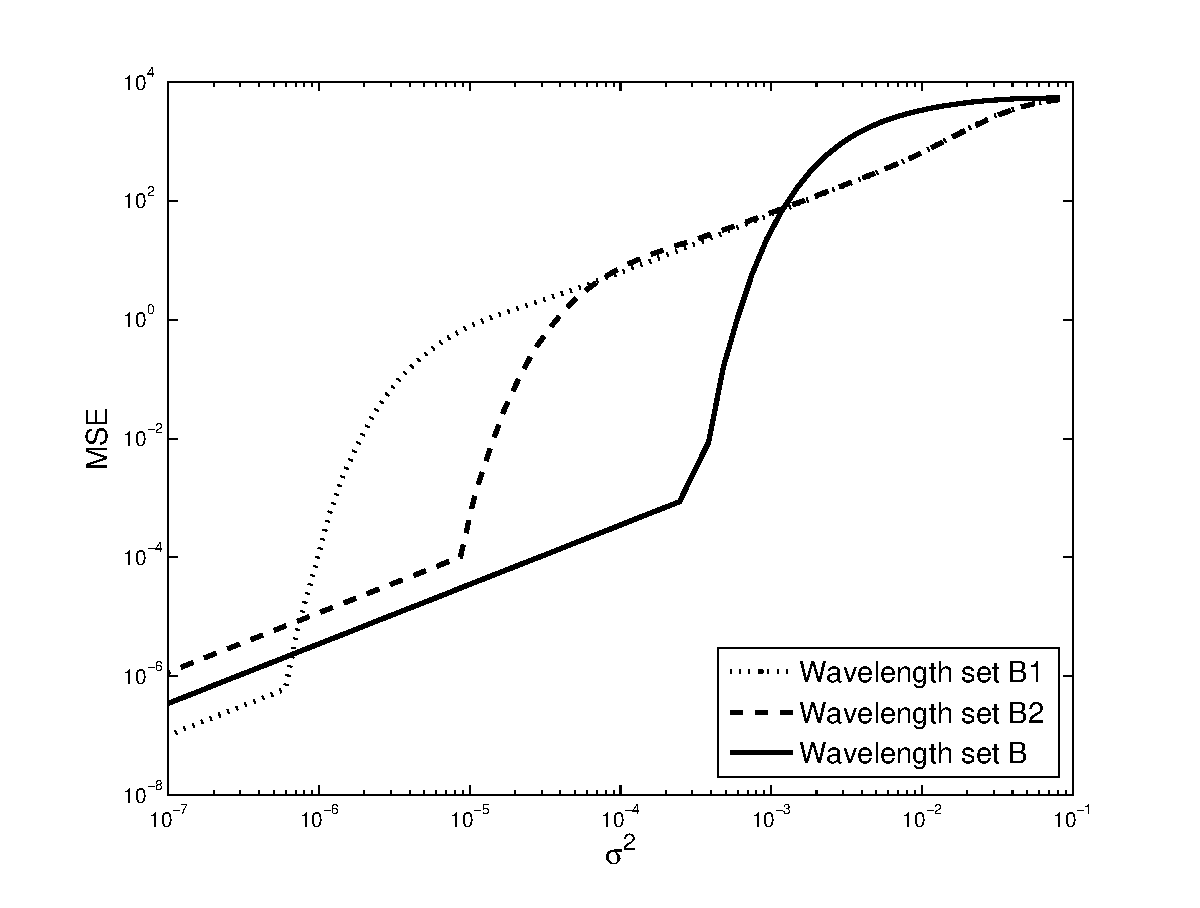
\includegraphics[scale=0.60]{code/data/Comparison_B1_B2_B.eps} 
% 		\caption{Effect of measurement wavelengths of the MSE curve.}     
% 		\label{fig:msecomparison}   
% \end{figure} 

%In Figure~{fig:benchmarks} we compare the computational complexity of the least squares range estimator with the CRT based range estimator. The computational complexity of the least squares range estimator (computed using a sphere decoder~\cite{Agrell2002}) grows exponentially with the number of wavelengths.  However, because the number of wavelengths is small in practice (we don't know of applications that use more than 10 wavelengths) computational complexity is not of serious concern. Figure~\ref{ch3:fig:benchmarks} shows the computation time required for the least squares estimator computed using a sphere decoder and the single stage CRT estimator of Xiao~et.~al.~\cite{Xiao_multistage_crt_2014} as the number of wavelengths $N$ increases.  The wavelengths are set to integers $\{1,2,3,\dots,N\}$ in each benchmark. In these benchmarks the least squares estimator is actually faster than the CRT for $N$ less than 38.  However, for large $N$ the sphere decoder becomes prohibitively expensive.
%
%
%\begin{figure}
%\centering
%  \begin{tikzpicture}
%    \selectcolormodel{gray} 
%    \begin{axis}[font=\footnotesize,ymode=log,height=11cm,width=14cm,xlabel={$N$},ylabel={time (ms)}, legend style={draw=none,fill=none,legend pos=north west,cells={anchor=west},font=\footnotesize}]
%      \addplot[mark= ] table {chapters/ch3/figs/LeastSquaresBenchmark};
%      \addplot[mark= ,dashed] table {chapters/ch3/figs/CRTBenchmark};
%      \legend{Least squares, CRT}
%   \end{axis}
%  \end{tikzpicture}  
% \caption{Computation time benchmark: Least squares estimator vs CRT estimator.}
% \label{ch3:fig:benchmarks}
%\end{figure} 



% The computational complexity mainly depends on the closest lattice point algorithm. This paper employs sphere decoder whereas \cite{Li_distance_est_wrapped_phase} used Babi's algorithm to find the closest lattice point.  As the number of wavelengths used in practical systems are usually less than ten (e.g. two for GPS) the sphere decoder's complexity is close to  the Babai's algorithm for low dimensions (less than ten). Furthermore, it has been noted that the proposed algorithm is faster than the CRT method proposed in~\cite{Xiao_multistage_crt_2014}.


 \section{Summary}
In this chapter, we considered the problem of estimating the range (or distance) between two locations using the phase of arrival method which provides the most accurate range estimates in many applications. A difficulty with phase of arrival is that only the principal component of the phase can be observed. This limits the range that can be unambiguously estimated to the wavelength of the signal. This problem is addressed by utilising signals of multiple different wavelengths and observing the phase at each. 

In this chapter we have considered least squares/maximum likelihood estimation of range from observation of phase at multiple wavelengths. We showed that the least squares range estimator can be computed by solving a problem from computational number theory known as the~\emph{closest lattice point problem}. Efficient general purpose algorithms for computing a closest lattice point require a~\emph{basis} for the lattice.  Constructing a basis for the least squares estimator of range is non-trivial. Bases have previously been constructed under the assumption that the wavelengths can be scaled to relatively prime integers.  In this chapter, interesting properties of lattices generated by intersection with or projection onto a subspace are used to construct a basis in the general case. Furthermore, the basis construction method provided in this research is simpler than the existing method provided in~\cite{Li_distance_est_wrapped_phase}. 

The construction of basis for the general case is important because the accuracy of the range estimator depends upon the wavelengths. Simulations indicate that this can dramatically improve range estimates.  These results lead to important problems of characterising the dependence of the least squares range estimator upon the measurement wavelengths and selecting wavelengths to maximise the accuracy of the least squares estimator that is addressed in the following chapters.





